\documentclass[11pt]{charter}
\usepackage[section]{placeins}
% El títulos de la memoria, se usa en la carátula y se puede usar el cualquier lugar del documento con el comando \ttitle
\titulo{Red de sensores WiFi para sistema productivo} 

% Nombre del posgrado, se usa en la carátula y se puede usar el cualquier lugar del documento con el comando \degreename
\posgrado{Carrera de Especialización en Sistemas Embebidos} 
%\posgrado{Carrera de Especialización en Internet de las Cosas} 
%\posgrado{Carrera de Especialización en Intelegencia Artificial}
%\posgrado{Maestría en Sistemas Embebidos} 
%\posgrado{Maestría en Internet de las cosas}

% Tu nombre, se puede usar el cualquier lugar del documento con el comando \authorname
\autor{Francisco G. Timez} 

% El nombre del director y co-director, se puede usar el cualquier lugar del documento con el comando \supname y \cosupname y \pertesupname y \pertecosupname
\director{Marcelo Pistarelli}
\pertenenciaDirector{UNR} 
% FIXME:NO IMPLEMENTADO EL CODIRECTOR ni su pertenencia
\codirector{} % si queda vacio no se deberíá incluir 
\pertenenciaCoDirector{}

% Nombre del cliente, quien va a aprobar los resultados del proyecto, se puede usar con el comando \clientename y \empclientename
\cliente{Pablo Scherf}
\empresaCliente{Cerámica FELI}

% Nombre y pertenencia de los jurados, se pueden usar el cualquier lugar del documento con el comando \jurunoname, \jurdosname y \jurtresname y \perteunoname, \pertedosname y \pertetresname.
\juradoUno{Nombre y Apellido (1)}
\pertenenciaJurUno{pertenencia (1)} 
\juradoDos{Nombre y Apellido (2)}
\pertenenciaJurDos{pertenencia (2)}
\juradoTres{Nombre y Apellido (3)}
\pertenenciaJurTres{pertenencia (3)}
 
\fechaINICIO{22 de junio de 2020}		%Fecha de inicio de la cursada de GdP \fechaInicioName
\fechaFINALPlanificacion{22 de Agosto de 2020} 	%Fecha de final de cursada de GdP
\fechaFINALTrabajo{22 de Julio de 2021}		%Fecha de defensa pública del trabajo final


\begin{document}

\maketitle
\thispagestyle{empty}
\pagebreak


\thispagestyle{empty}
{\setlength{\parskip}{0pt}
\tableofcontents{}
}
\pagebreak


\section{Registros de cambios}
\label{sec:registro}


\begin{table}[ht]
\label{tab:registro}
\centering

\begin{tabularx}{\linewidth}{@{}|c|X|c|@{}}
\hline
\rowcolor[HTML]{C0C0C0} 
Revisión & \multicolumn{1}{c|}{\cellcolor[HTML]{C0C0C0}Detalles de los cambios realizados} & Fecha      \\ \hline
1.0      & Creación del documento                                                          & 22/06/2020 \\ \hline
1.1      & Avances hasta capítulo 6. Desglose de tareas									   & 10/07/2020 \\ \hline
1.2      & Se atendieron a las correcciones enviadas el día 14/07/2020                     & 15/07/2020 \\ \hline
1.3      & Avances hasta capítulo 11. Matriz de asignación de responsabilidades            & 30/07/2020 \\ \hline
1.4      & Avances hasta capítulo 17. Procesos de cierre          						   & 08/08/2020 \\ \hline
1.5      & Se atendieron a las correcciones enviadas el día 09/08/2020. Se agregan historias de usuario.	& 14/08/2020 \\ \hline
\end{tabularx}
\end{table}

\pagebreak



\section{Acta de constitución del proyecto}
\label{sec:acta}

\begin{flushright}
Buenos Aires, \fechaInicioName
\end{flushright}

\vspace{2cm}

Por medio de la presente se acuerda con el Ing. \authorname\hspace{1px} que su Trabajo Final de la \degreename\hspace{1px} se titulará ``\ttitle'', consistirá esencialmente en el prototipo preliminar de un sensor de fácil configuración e instalación, para el registro de datos ambientales o de procesos específicos, y tendrá un presupuesto preliminar estimado en 640 hs y un costo estimado en xxxx pesos argentinos, con fecha de inicio \fechaInicioName\hspace{1px} y fecha de presentación pública \fechaFinalName.

Se adjunta a esta acta la planificación inicial.

\vfill

% Esta parte se construye sola con la información que hayan cargado en el preámbulo del documento y no debe modificarla
\begin{table}[ht]
\centering
\begin{tabular}{ccc}
\begin{tabular}[c]{@{}c@{}}Ariel Lutenberg \\ Director posgrado FIUBA\end{tabular} &  & \begin{tabular}[c]{@{}c@{}}\clientename \\ \empclientename \end{tabular} \vspace{2.5cm} \\ 
\multicolumn{3}{c}{\begin{tabular}[c]{@{}c@{}} \supname \\ Director del Trabajo Final\end{tabular}} \vspace{2.5cm} \\
\begin{tabular}[c]{@{}c@{}}\jurunoname \\ Jurado del Trabajo Final\end{tabular}     &  & \begin{tabular}[c]{@{}c@{}}\jurdosname\\ Jurado del Trabajo Final\end{tabular}  \vspace{2.5cm}  \\
\multicolumn{3}{c}{\begin{tabular}[c]{@{}c@{}} \jurtresname\\ Jurado del Trabajo Final\end{tabular}} \vspace{.5cm}                                                                     
\end{tabular}
\end{table}




\section{Descripción técnica-conceptual del proyecto a realizar}
\label{sec:descripcion}


En las PyMEs dedicadas a la industria ceramista, en la mayoría de las situaciones los emprendedores corrigen, a prueba y error, los parámetros de sus procesos productivos en base a los resultados obtenidos de la producción. Las correcciones se realizan según la experiencia propia del emprendedor y en la mayoría de los casos no se realizan registro de las variables del proceso.

Partiendo de la premisa que “lo que no se puede medir, no se puede mejorar”, se propone un sistema de fácil configuración e instalación, que les permita a estos emprendedores, en un principio, utilizar los criterios formados en la experiencia, y poder darles una base sólida en los datos para poder mejorar de manera continua.

Este proyecto debe ser de implementación sencilla, por dos motivos. Primero, no suelen tener un departamento dentro de la PyME dedicado al mantenimiento, pero si personal con conocimientos de electricidad industrial. Segundo, la estructura edilicia de la industria se modifica constantemente. Entonces debe ser un producto que se pueda reinstalar en otro sitio sin mayores inconvenientes.

Uno de los desafíos más importantes de este proyecto radica en reducir los costos de implementación, tiene que permitirle a la PyME instalar, desinstalar y reubicar los sensores con recursos propios, sin recurrir a mano de obra especializada.

El sistema consiste en nodos que se desarrollan en forma genérica y que pueden ser configurados según la necesidad de la PyME. Como se puede ver en la figura \ref{fig:diagBloques}, los nodos son similares, pero pueden tener distintas funciones asignadas, el Nodo 01 sensa temperatura y humedad, el Nodo 02 sensa temperatura y un switch (podría funcionar como contador) y el Nodo 03 tiene un módulo de expansión I2C. De esta manera, si algún Nodo pierde utilidad en el lugar donde se encuentra instalado, puede ser reubicado cambiando su configuración o no.


\vspace{10px}

\begin{figure}[htpb]
\centering 
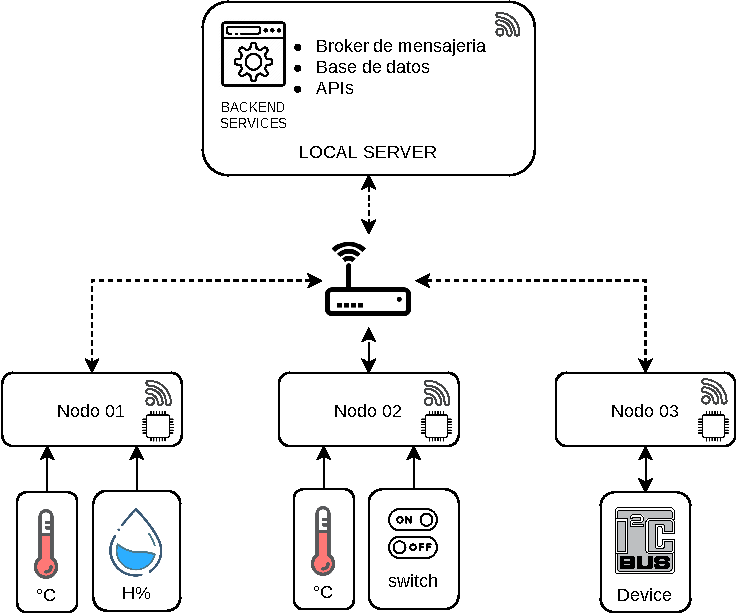
\includegraphics[width=.68\textwidth]{./Figuras/DiagramaEnBloques.pdf}
\caption{Diagrama en bloques del sistema}
\label{fig:diagBloques}
\end{figure}

\vspace{10px}


\section{Identificación y análisis de los interesados}
\label{sec:interesados}

\begin{table}[ht]
%\caption{Identificación de los interesados}
%\label{tab:interesados}
\begin{tabularx}{\linewidth}{@{}|l|X|X|l|@{}}
\hline
\rowcolor[HTML]{C0C0C0} 
Rol				& Nombre y Apellido & Organización 		& Puesto 	\\ \hline
Auspiciante		&					&					&			\\
Cliente			& \clientename      & \empclientename	& Gerente  	\\ 
Impulsor		&					&					&			\\	\hline
Responsable		& \authorname       & FIUBA        		& Alumno 	\\ \hline
Orientador		& \supname	      	& \pertesupname 	& Director	Trabajo final \\ \hline
Usuario final	& Personal técnico  & PyME           	& -       	\\ \hline
\end{tabularx}
\end{table}

\section{1. Propósito del proyecto}
\label{sec:proposito}

El propósito de este proyecto es brindarle a la PyME un recurso técnico económico para lograr implementar un sistema de seguimiento a su proceso o línea productiva; que le permita sensar variables de producción y tener los datos disponibles en gráficos actualizados en tiempo real.

\section{2. Alcance del proyecto}
\label{sec:alcance}

El desarrollo del presente proyecto incluye:
\begin{itemize}
\item Análisis, investigación y elección del hardware para el nodo.
\item Desarrollo de un prototipo de nodo que soporte distintos sensores detallados en los requerimientos.
\item Desarrollo del firmware del nodo.
\item Software \textit{backend} para almacenar los datos de los sensores en una base de datos tipo SQL.
\item Instalación de una interfaz gráfica estándar para visualización de los datos almacenados en la base de datos.
\end{itemize}

El proyecto NO incluye:
\begin{itemize}
\item Desarrollo de una interfaz web o gráfica específica para interactuar con los datos.
\item Desarrollo de una interfaz gráfica para configuración de los nodos.
\item Desarrollo de módulos de sensores para el nodo.
\item Pruebas de validación en campo.
\end{itemize}


\section{3. Supuestos del proyecto}
\label{sec:supuestos}

Para el desarrollo del presente proyecto se supone que:

\begin{itemize}
\item Los componentes electrónicos necesarios se consiguen dentro de territorio Argentino.
\item Se realizará un solo proceso de compra.
\item Los sensores son todos con salida digital, se supone que no requieren un proceso de calibración y ajuste.
\item La estructura de red WiFi existe y está en funcionamiento en la PyME.
\item La cobertura de la red WiFi es la adecuada para la línea productiva de la PyME.
\end{itemize}

\section{4. Requerimientos}
\label{sec:requerimientos}

Requerimientos del proyecto:


\begin{enumerate}
\item Requerimientos de hardware del nodo:
	\begin{enumerate}
	\item Debe soportar tensiones de alimentación de 5 Vdc a 24 Vdc.
	\item Debe basarse en el microcontrolador ESP8266 ó ESP32.
	\item Debe tener puerto de I2C para conectar otros módulos de expansión.
	\item Entradas:
		\begin{enumerate}
		\item Sensor de temperatura y humedad DHT22.
		\item Sensor de temperatura termopar K con MAX6675.
		\item Al menos una entrada para sensores con salida relé o transistorizados NPN.
		\end{enumerate}
	\end{enumerate}
\item Requerimientos de firmware del nodo:
	\begin{enumerate}
	\item Comunicación WiFi y por protocolo MQTT.
	\item Se debe poder configurar los sensores mediante un archivo JSON, con posibilidad de actualización mediante OTA.
	\item Se debe soportar actualización del firmware mediante OTA.
	\item Se debe soportar el módulo de expansión PCF8574.
	\end{enumerate}
\item Requerimientos de software backend:
	\begin{enumerate}
	\item Todos los servicios deben correr en una Raspberry Pi 3 o 4.
	\item Broker MQTT alojado en red local.
	\item Backend basado en Node-RED o NodeJS.
	\item Generación de tablas en base de datos SQL, según configuración del nodo.
	\item Dashboard web de variables sensadas mediante Grafana.
	\end{enumerate}
\end{enumerate}

\section{Historias de usuarios (\textit{Product backlog})}
\label{sec:backlog}
Las siguientes historias de usuario se utiliza el siguiente criterio:
\begin{itemize}
\item Ponderación: 1 esfuerzo bajo, 3 esfuerzo moderado, 7 esfuerzo alto.
\item Prioridad: 1 alta, 2 media, 3 baja.
\end{itemize}

Como gerente, quiero ver en una pantalla dos datos de los sensores.
\begin{itemize}
\item Ponderación: 1.
\item Prioridad: 3.
\end{itemize}

Como técnico, quiero configurar el nodo con un archivo de texto.
\begin{itemize}
\item Ponderación: 7.
\item Prioridad: 2.
\end{itemize}

Como técnico, quiero actualizar la configuración del nodo con un archivo de texto.
\begin{itemize}
\item Ponderación: 7.
\item Prioridad: 3.
\end{itemize}

Como técnico, quiero conectar una termocupla tipo K al nodo.
\begin{itemize}
\item Ponderación: 3.
\item Prioridad: 1.
\end{itemize}

Como técnico, quiero conectar un sensor de temperatura y humedad al nodo.
\begin{itemize}
\item Ponderación: 1.
\item Prioridad: 1.
\end{itemize}

Como técnico, quiero agregar mas entradas tipo switch al nodo.
\begin{itemize}
\item Ponderación: 7.
\item Prioridad: 2.
\end{itemize}




\section{5. Entregables principales del proyecto}
\label{sec:entregables}

\begin{itemize}
\item Manual de configuración
\item Diagrama esquemático
\item Código fuente
\item Informe final
\end{itemize}

\section{6. Desglose del trabajo en tareas}
\label{sec:wbs}

\begin{enumerate}
\item Planificación del Proyecto (40 hs)
	\begin{enumerate}
	\item Elaboración del documento de planificación del proyecto (20 hs)
	\item Diseño de la arquitectura global del proyecto (20 hs)
	\end{enumerate}
\item Desarrollo del hardware del nodo (150 hs)
	\begin{enumerate}
	\item Diseño del diagrama esquemático (40 hs)
	\item Selección y compra de componentes (20 hs)
	\item Routeo PCB (40 hs)
	\item Fabricación del PCB (30 hs)
	\item Verificación y testing básico del prototipo (20 hs)
	\end{enumerate}
\item Desarrollo del firmware del nodo (210 hs)
	\begin{enumerate}
	\item Tests con freeRTOS (50 hs)
		\begin{enumerate}
		\item Generar tareas con los parámetros cargados desde un archivo JSON (25 hs)
		\item Actualización de tareas con la actualización del archivo JSON (25 hs)
		\end{enumerate}
	\item Diseño de la arquitectura de software (20 hs)
	\item Desarrollo de tareas para comunicación WiFi con broker de mensajería (20 hs)
	\item Desarrollo de las tareas para gestión de sensores (40 hs)
	\item Desarrollo de las tareas para gestión de puerto de expansión I2C (40 hs)
	\item Integración de todas las tareas desarrolladas (40 hs)
	\end{enumerate}
\item Desarrollo del backend (240 hs)
\begin{enumerate}
	\item Diseño de la arquitectura de software (40 hs)
	\item Instalación de broker de mensajería (20 hs)
	\item Instalación de base de datos (20 hs)
	\item Desarrollo software de backend (100 hs)
		\begin{enumerate}
		\item Introducción a NodeJS (50 hs)
		\item Desarrollo bloque para comunicación con broker de mensajería (25 hs)
		\item Desarrollo bloque para inserción de datos en la base de datos (25 hs)
		\end{enumerate}
	\item Instalación y configuración de Grafana (20 hs)
	\item Integración de los bloques desarrollados (40 hs)
	\end{enumerate}
\end{enumerate}


Cantidad total de horas: (640 hs)

\clearpage

\section{7. Diagrama de Activity On Node}
\label{sec:AoN}

En el diagrama de Activity On Node se utiliza ``hora'' como unidad de tiempo y las flechas gruesas marcan el camino crítico del proyecto.

%La figura \ref{fig:AoN} fue elaborada con el paquete latex tikz y pueden consultar la siguiente referencia \textit{online}:

%\url{https://www.overleaf.com/learn/latex/LaTeX_Graphics_using_TikZ:_A_Tutorial_for_Beginners_(Part_3)\%E2\%80\%94Creating_Flowcharts}


\begin{figure}[htpb]
\centering 
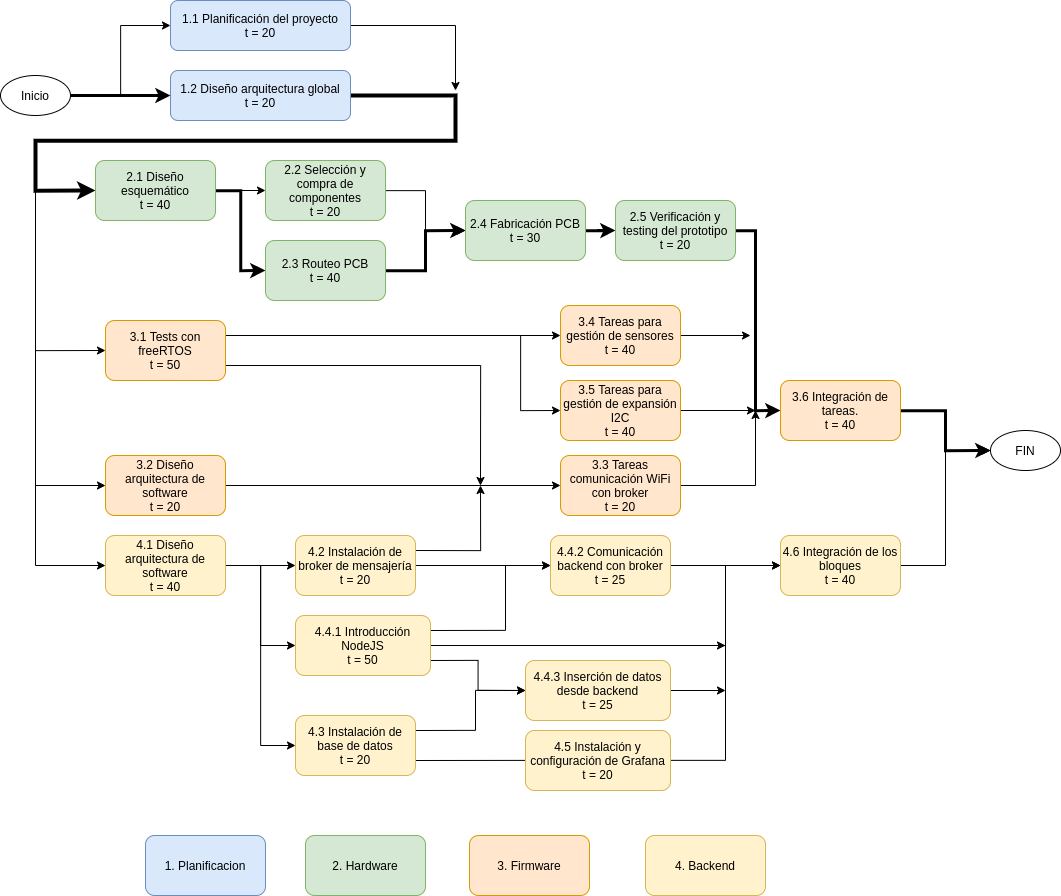
\includegraphics[width=\textwidth]{./Figuras/AoN.png}
\caption{Diagrama en \textit{Activity on Node}}
\label{fig:AoN}
\end{figure}

\clearpage

\section{8. Diagrama de Gantt}
\label{sec:gantt}
En el diagrama de Gantt se supone que al proyecto se le dedicará 2 horas de trabajo por día, los 7 días de la semana. La cantidad de horas de trabajo por día es un estimativo promedio mensual. De esta forma la unidad de tiempo en el diagrama de Gantt es ``día''.

\begin{figure}[htpb]
\centering 
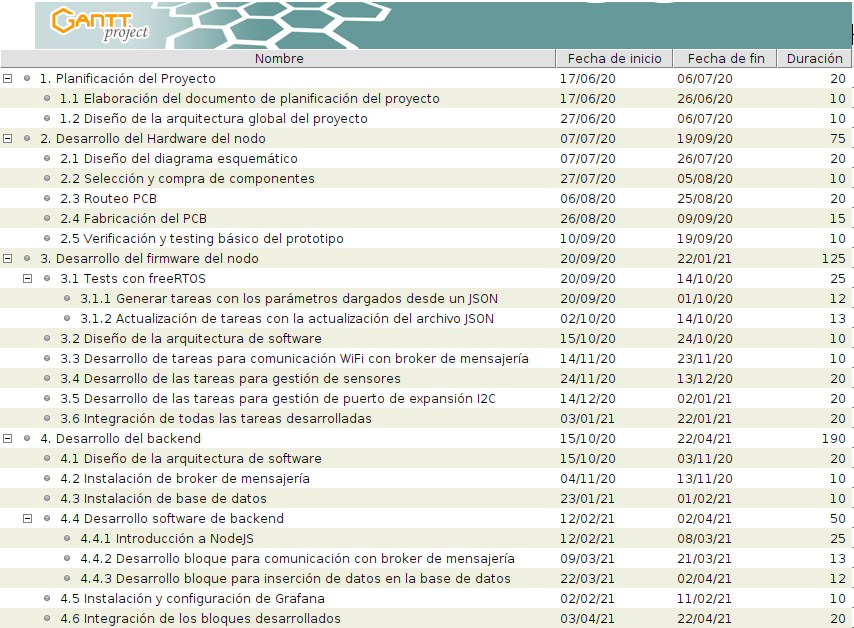
\includegraphics[width=\textwidth]{./Figuras/TabGanttRedSensores.png}
\caption{Diagrama de \textit{Gantt}}
\label{fig:TabGantt}
\end{figure}

\begin{figure}[htb]
\centering 
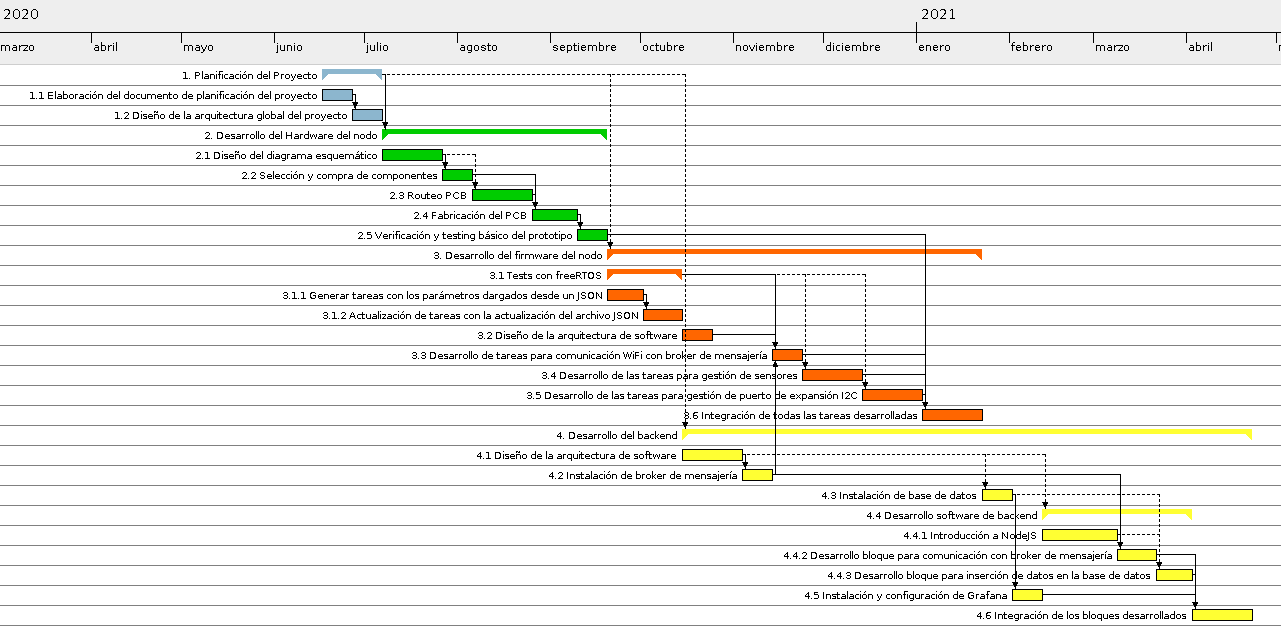
\includegraphics[angle=90, height=.96\textheight]{./Figuras/GanttRedSensores2.png}
\caption{Diagrama de \textit{Gantt} (Gráfico)}
\label{fig:Gantt}
\end{figure}

\section{9. Matriz de uso de recursos de materiales}
\label{sec:recursos}


% Please add the following required packages to your document preamble:
% \usepackage{multirow}
% \usepackage{graphicx}
% \usepackage[table,xcdraw]{xcolor}
% If you use beamer only pass "xcolor=table" option, i.e. \documentclass[xcolor=table]{beamer}
\begin{table}[ht]
\centering
\resizebox{\textwidth}{!}{%
\begin{tabular}{|l|l|c|c|c|c|c|}
\hline
\rowcolor[HTML]{C0C0C0} 
\multicolumn{1}{|c|}{\cellcolor[HTML]{C0C0C0}} &
  \multicolumn{1}{c|}{\cellcolor[HTML]{C0C0C0}} &
  \multicolumn{5}{c|}{\cellcolor[HTML]{C0C0C0}Recursos requeridos (horas)} \\ \cline{3-7} 
\multicolumn{1}{|c|}{\multirow{-2}{*}{\cellcolor[HTML]{C0C0C0}\begin{tabular}[c]{@{}c@{}}código \\ WBS\end{tabular}}} &
  \multicolumn{1}{c|}{\multirow{-2}{*}{\cellcolor[HTML]{C0C0C0}Nombre tarea}} &
  PC &
  \begin{tabular}[c]{@{}c@{}}Raspberry\\ Pi\end{tabular} &
  Laboratorio &
  \begin{tabular}[c]{@{}c@{}}Kit de\\ desarrollo\end{tabular} &
  PCB \\ \hline
\rowcolor[HTML]{EFEFEF} 
1     & Planificación del Proyecto                                           & \multicolumn{5}{c|}{\cellcolor[HTML]{EFEFEF}} \\ \hline
1.1   & Elaboración del documento de planificación del proyecto              & 20      &         &         &        &        \\ \hline
1.2   & Diseño de la arquitectura global del proyecto                        & 20      &         &         &        &        \\ \hline
\rowcolor[HTML]{EFEFEF} 
2     & Desarrollo del hardware del nodo                                     & \multicolumn{5}{c|}{\cellcolor[HTML]{EFEFEF}} \\ \hline
2.1   & Diseño del diagrama esquemático                                      & 40      &         &         &        &        \\ \hline
2.2   & Selección y compra de componentes                                    & 20      &         &         &        &        \\ \hline
2.3   & Routeo PCB                                                           & 40      &         &         &        &        \\ \hline
2.4   & Fabricación del PCB                                                  & 5       &         & 25      &        &        \\ \hline
2.5   & Verificación y testing básico del prototipo                          & 20      &         & 20      &        &        \\ \hline
\rowcolor[HTML]{EFEFEF} 
3     & Desarrollo del firmware del nodo                                     & \multicolumn{5}{c|}{\cellcolor[HTML]{EFEFEF}} \\ \hline
3.1   & Tests con freeRTOS                                                   & 50      &         &         & 50     &        \\ \hline
3.2   & Diseño de la arquitectura de software                                & 20      &         &         &        &        \\ \hline
3.3   & Desarrollo de tareas para comunicación WiFi con broker de mensajería & 20      & 20      &         &        &        \\ \hline
3.4   & Desarrollo de las tareas para gestión de sensores                    & 40      &         &         & 40     &        \\ \hline
3.5   & Desarrollo de las tareas para gestión de puerto de expansión I2C     & 40      &         &         & 40     &        \\ \hline
3.6   & Integración de todas las tareas desarrolladas                        & 40      &         &         &        & 40     \\ \hline
\rowcolor[HTML]{EFEFEF} 
4     & Desarrollo del backend                                               & \multicolumn{5}{c|}{\cellcolor[HTML]{EFEFEF}} \\ \hline
4.1   & Diseño de la arquitectura de software                                & 40      &         &         &        &        \\ \hline
4.2   & Instalación de broker de mensajería                                  & 20      & 20      &         &        &        \\ \hline
4.3   & Instalación de base de datos                                         & 20      & 20      &         &        &        \\ \hline
4.4   & Desarrollo software de backend                                       & \multicolumn{5}{c|}{}                         \\ \hline
4.4.1 & Introducción a NodeJS                                                & 50      &         &         &        &        \\ \hline
4.4.2 & Desarrollo bloque para comunicación con broker de mensajería         & 25      & 25      &         &        &        \\ \hline
4.4.3 & Desarrollo bloque para inserción de datos en la base de datos        & 25      & 25      &         &        &        \\ \hline
4.5   & Instalación y configuración de Grafana                               & 20      & 20      &         &        &        \\ \hline
4.6   & Integración de los bloques desarrollados                             & 40      & 40      &         &        & 40     \\ \hline
\rowcolor[HTML]{9B9B9B} 
 &
  Total de horas por recurso &
  \multicolumn{1}{c|}{\cellcolor[HTML]{9B9B9B}615} &
  \multicolumn{1}{c|}{\cellcolor[HTML]{9B9B9B}170} &
  \multicolumn{1}{c|}{\cellcolor[HTML]{9B9B9B}45} &
  \multicolumn{1}{c|}{\cellcolor[HTML]{9B9B9B}130} &
  \multicolumn{1}{c|}{\cellcolor[HTML]{9B9B9B}80} \\ \hline
\end{tabular}%
}
\end{table}


\section{10. Presupuesto detallado del proyecto}
\label{sec:presupuesto}


% Please add the following required packages to your document preamble:
% \usepackage{graphicx}
% \usepackage[table,xcdraw]{xcolor}
% If you use beamer only pass "xcolor=table" option, i.e. \documentclass[xcolor=table]{beamer}
\begin{table}[htpb]
\centering
\resizebox{0.7\textwidth}{!}{%
\begin{tabular}{|l|l|l|l|}
\hline
\rowcolor[HTML]{9B9B9B} 
\multicolumn{4}{|l|}{\cellcolor[HTML]{9B9B9B}COSTOS DIRECTOS}      \\ \hline
\rowcolor[HTML]{9B9B9B} 
Descripcion             & Cantidad & Valor unitario & Valor total  \\ \hline
Trabajo directo         & 640 hs   & \$750,00       & \$480.000,00 \\ \hline
Raspberry Pi            & 1        & \$15.000,00    & \$15.000,00  \\ \hline
Fabricacion del PCB     & 10       & \$5.000,00     & \$50.000,00  \\ \hline
Kit de desarrollo       & 2        & \$3.000,00     & \$6.000,00   \\ \hline
\multicolumn{3}{|l|}{SUBTOTAL}                      & \$551.000,00 \\ \hline
\rowcolor[HTML]{9B9B9B} 
\multicolumn{4}{|l|}{\cellcolor[HTML]{9B9B9B}COSTOS INDIRECTOS}    \\ \hline
\rowcolor[HTML]{9B9B9B} 
Descripcion             & Cantidad & Valor unitario & Valor total  \\ \hline
30\% de trabajo directo & 192 hs   & \$750,00       & \$144.000,00 \\ \hline
\multicolumn{3}{|l|}{SUBTOTAL}                      & \$144.000,00 \\ \hline
\rowcolor[HTML]{9B9B9B} 
\multicolumn{3}{|l|}{\cellcolor[HTML]{9B9B9B}TOTAL} & \$695.000,00 \\ \hline
\end{tabular}%
}
\end{table}

\section{11. Matriz de asignación de responsabilidades}
\label{sec:responsabilidades}

% Please add the following required packages to your document preamble:
% \usepackage{multirow}
% \usepackage{graphicx}
% \usepackage[table,xcdraw]{xcolor}
% If you use beamer only pass "xcolor=table" option, i.e. \documentclass[xcolor=table]{beamer}
\begin{table}[htpb]
\centering
\resizebox{\textwidth}{!}{%
\begin{tabular}{|l|l|c|c|c|}
\hline
\rowcolor[HTML]{9B9B9B} 
\multicolumn{1}{|c|}{\cellcolor[HTML]{9B9B9B}} &
  \multicolumn{1}{c|}{\cellcolor[HTML]{9B9B9B}} &
  Responsable &
  Orientador &
  Cliente \\ \cline{3-5} 
\rowcolor[HTML]{9B9B9B} 
\multicolumn{1}{|c|}{\multirow{-2}{*}{\cellcolor[HTML]{9B9B9B}\begin{tabular}[c]{@{}c@{}}código\\ WBS\end{tabular}}} &
  \multicolumn{1}{c|}{\multirow{-2}{*}{\cellcolor[HTML]{9B9B9B}Nombre tarea}} &
  \begin{tabular}[c]{@{}c@{}}Francisco\\Timez\end{tabular} &
  \begin{tabular}[c]{@{}c@{}}Marcelo\\Pistarelli\end{tabular} &
  \begin{tabular}[c]{@{}c@{}}Pablo\\Scherf\end{tabular}\\ \hline
1        & \multicolumn{4}{l|}{Planificación del Proyecto}                                   \\ \hline
1.1      & Elaboración del documento de planificación del proyecto               & P & A & I \\ \hline
1.2      & Diseño de la arquitectura global del proyecto                         & P & I & I \\ \hline
2        & \multicolumn{4}{l|}{Desarrollo del hardware del nodo}                             \\ \hline
2.1      & Diseño del diagrama esquemático                                       & P &   & C \\ \hline
2.2      & Selección y compra de componentes                                     & P &   & A \\ \hline
2.3      & Routeo PCB                                                            & P &   &   \\ \hline
2.4      & Fabricación del PCB                                                   & P &   & I \\ \hline
2.5      & Verificación y testing básico del prototipo                           & P &   & A \\ \hline
3        & \multicolumn{4}{l|}{Desarrollo del firmware del nodo}                             \\ \hline
3.1      & \multicolumn{4}{l|}{Tests con freeRTOS}                                           \\ \hline
3.1.1	 & Generar tareas con los parámetros cargados desde un archivo JSON      & P &   &   \\ \hline
3.1.2	 & Actualización de tareas con la actualización del archivo JSON         & P &   &   \\ \hline
3.2      & Diseño de la arquitectura de software                                 & P & C &   \\ \hline
3.3      & Desarrollo de tareas para comunicación WiFi con broker de mensajería & P & I &   \\ \hline
3.4      & Desarrollo de las tareas para gestión de sensores                     & P & I &   \\ \hline
3.5      & Desarrollo de las tareas para gestión de puerto de expansión I2C      & P & I &   \\ \hline
3.6      & Integración de todas las tareas desarrolladas                         & P & I & I \\ \hline
4        & \multicolumn{4}{l|}{Desarrollo del backend}                                       \\ \hline
4.1      & Diseño de la arquitectura de software                                 & P & C &   \\ \hline
4.2      & Instalación de broker de mensajería                                  & P &   &   \\ \hline
4.3      & Instalación de base de datos                                          & P &   & C \\ \hline
4.4      & \multicolumn{4}{l|}{Desarrollo software de backend}                               \\ \hline
4.4.1    & Introducción a NodeJS                                                 & P &   &   \\ \hline
4.4.2    & Desarrollo bloque para comunicación con broker de mensajería         & P &   &   \\ \hline
4.4.3    & Desarrollo bloque para inserción de datos en la base de datos         & P &   &   \\ \hline
4.5      & Instalación y configuración de Grafana                                & P &   & A \\ \hline
4.6      & Integración de los bloques desarrollados                              & P & I & I \\ \hline
\end{tabular}%
}
\end{table}

{\footnotesize
Referencias:
\begin{itemize}
	\item P = Responsabilidad Primaria
	\item S = Responsabilidad Secundaria
	\item A = Aprobación
	\item I = Informado
	\item C = Consultado
\end{itemize}
} %footnotesize

\section{12. Gestión de riesgos}
\label{sec:riesgos}

A continuación se describen los riesgos asociados al proyecto, junto con un plan de mitigación a los fines de reducir la probabilidad de errores.

a) Identificación de los riesgos

\begin{itemize}
\item Riesgo 1: falta de tiempo para la finalización del proyecto.
	\begin{itemize}
	\item Severidad (9): implicaría no terminar la especialización en sistemas embebidos.
	\item Probabilidad de ocurrencia (3): se cuenta con una planificación detallada del proyecto. 
	\end{itemize} 

\item Riesgo 2: retraso en el desarrollo de software de backend.
	\begin{itemize}
	\item Severidad (8): debido a la capacidad técnica actual, esto puede retrasar la finalización del proyecto.
	\item Probabilidad de ocurrencia (10): alta debido a que no se posee experiencia en el desarrollo de software de backend. 
	\end{itemize}
	
\item Riesgo 3: pérdida de archivos por falla, rotura o robo de las herramientas de desarrollo (Computadora Personal)
	\begin{itemize}
	\item Severidad (8): implicaría perder gran parte del trabajo, junto con su documentación.
	\item Probabilidad de ocurrencia (5): probabilidad media debido a que me movilizo con la computadora por la ciudad y además tiene acumulada muchas horas de uso.
	\end{itemize}
	
\item Riesgo 4: no conseguir los componentes necesarios para el proyecto.
	\begin{itemize}
	\item Severidad (5): implicaría volver a la etapa de diseño del PCB.
	\item Probabilidad de ocurrencia (5): hay pocos importadores de componentes electrónicos en el país, y traer a pedido implica una demora no aceptable para el proyecto.
	\end{itemize}
	
\item Riesgo 5: falla en el PCB.
	\begin{itemize}
	\item Severidad (5): demoraría las pruebas de integración del proyecto.
	\item Probabilidad de ocurrencia (5): al ser de fabricación artesanal pueden ocurrir cortocircuitos en las pistas con elementos extraños o errores en el revelado del PCB. 
	\end{itemize}
\end{itemize} 

b) Tabla de gestión de riesgos: (El RPN se calcula como RPN=SxO)

\begin{table}[htpb]
\centering
\begin{tabularx}{\linewidth}{@{}|X|c|c|c|c|c|c|@{}}
\hline
\rowcolor[HTML]{C0C0C0} 
Riesgo & S & O & RPN & S* & O* & RPN* \\ \hline
Riesgo 1: falta de tiempo para la finalización del proyecto. & 9  & 3  & 27 &    &    &      \\ \hline
Riesgo 2: retraso en el desarrollo de software de backend. & 8  & 10 & 80 & 4  & 5  & 20   \\ \hline
Riesgo 3: pérdida de archivos por falla, rotura o robo de las herramientas de desarrollo (Computadora Personal) & 8  & 5  & 40 & 2  & 5  & 10   \\ \hline
Riesgo 4: no conseguir los componentes necesarios para el proyecto. & 5  & 5  & 25 &    &    &      \\ \hline
Riesgo 5: falla en el PCB. & 5  & 5  & 25 &    &    &      \\ \hline
\end{tabularx}%
\end{table}

Criterio adoptado: 
Se tomarán medidas de mitigación en los riesgos cuyos números de RPN sean mayores a 30.

Nota: los valores marcados con (*) en la tabla corresponden luego de haber aplicado la mitigación.

c) Plan de mitigación de los riesgos que originalmente excedían el RPN máximo establecido:

\begin{itemize}
\item Riesgo 2: se utilizará como recursos cursos virtuales en plataformas como udemy, Platzi, códigofacilito, EducaciónIT o similares.
	\begin{itemize}
	\item Severidad (4): se reduce la severidad debido a que se seguirá un plan de estudios, por lo tanto se reduce el tiempo de aprendizaje.
	\item Probabilidad de ocurrencia (5): tener un plan de estudio reduce la probabilidad de ocurrencia ya que se generan objetivos intermedios agilizando la tarea. 
	\end{itemize}
\item Riesgo 3: se utilizará un sistema de control de versiones en la nube, como por ejemplo Git y GitHub. Y se generarán alarmas para recordar de generar un guardado en la nube cada una semana.
	\begin{itemize}
	\item Severidad (2): luego de la mitigación se reduce notoriamente la severidad ya que se perderá como máximo el trabajo de una semana.
	\item Probabilidad de ocurrencia (5): la probabilidad de ocurrencia se mantiene debido a que depende de factores externos. 
	\end{itemize}
\end{itemize}  
 

\section{13. Gestión de la calidad}
\label{sec:calidad}

\begin{enumerate}
\item Requerimientos de hardware del nodo:
	\begin{enumerate}
	\item Debe soportar tensiones de alimentación de 5 Vdc a 24 Vdc.
		\\Verificación y validación:
		\begin{itemize}
		\item Verificación: se obtendrán de las hojas de datos de los componentes reguladores las tensiones máximas admitidas. 
		\item Validación: se energizará el dispositivo con una fuente de corriente continua regulable, desde los 5Vdc hasta los 24Vdc en incrementos de 1V. 
		\end{itemize}
	\item Debe basarse en el microcontrolador ESP8266 ó ESP32.
	\\Verificación y validación:
		\begin{itemize}
		\item Verificación: se analizarán los costos y las características de cada microcontrolador y se elegirá el que mejor se ajuste al proyecto.
		\item Validación: se harán testeos con placas de desarrollo.
		\end{itemize}
	\item Debe tener puerto de I2C para conectar otros módulos de expansión.
		\\Verificación y validación:
		\begin{itemize}
		\item Verificación: se investigará documentación del protocolo I2C para implementarlo correctamente.
		\item Validación: se harán testeos con placas de desarrollo y dispositivos I2C.
		\end{itemize}
	\item Entradas:
		\begin{enumerate}
		\item Sensor de temperatura y humedad DHT22.
			\\Verificación y validación:
			\begin{itemize}
			\item Verificación: se analizará la hoja de datos del sensor verificando las condiciones de funcionamiento.
			\item Validación: se realizarán testeos del sensor.
			\end{itemize}
		\item Sensor de temperatura termopar K con MAX6675.
			\\Verificación y validación:
			\begin{itemize}
			\item Verificación: se analizará la hoja de datos del CI conversor verificando las condiciones de funcionamiento.
			\item Validación: se realizarán testeos con distintas termocuplas comparando las mediciones con sensores digitales como Ds18b20.
			\end{itemize}
		\item Al menos una entrada para sensores con salida relé o transistorizados NPN.
			\\Verificación y validación:
			\begin{itemize}
			\item Verificación: se analizarán distintos tipos de sensores para verificar las condiciones de funcionamiento.
			\item Validación: se harán testeos con sensores industriales disponibles.
			\end{itemize}
		\end{enumerate}
	\end{enumerate}
\item Requerimientos de firmware del nodo:
	\begin{enumerate}
	\item Comunicación WiFi y por protocolo MQTT.
		\\Verificación y validación:
		\begin{itemize}
		\item Verificación: se verifica mediante la hoja de datos del dispositivo y documentación necesaria.
		\item Validación: se harán testeos enviando y recibiendo datos.
		\end{itemize}
	\item Se debe poder configurar los sensores mediante un archivo JSON, con posibilidad de actualización mediante OTA.
		\\Verificación y validación:
		\begin{itemize}
		\item Verificación: se construye un archivo JSON que contemple las configuraciones necesarias para las tareas.
		\item Validación: se harán testeos con creando, actualizando y borrando tareas.
		\end{itemize}
	\item Se debe soportar actualización del firmware mediante OTA.
		\\Verificación y validación:
		\begin{itemize}
		\item Verificación: se analizará la documentación para la implementación de OTA por HTTP.
		\item Validación: se harán testeos de actualización de firmware.
		\end{itemize}
	\item Se debe soportar el módulo de expansión PCF8574.
		\\Verificación y validación:
		\begin{itemize}
		\item Verificación: se analizará la hoja de datos del chip y se comprobará sus condiciones de funcionamiento.
		\item Validación: se harán testeos con al menos un modulo de expansión.
		\end{itemize}
	\end{enumerate}
\item Requerimientos de software backend:
	\begin{enumerate}
	\item Todos los servicios deben correr en una Raspberry Pi 3 o 4.
		\\Verificación y validación:
		\begin{itemize}
		\item Verificación: se verificará en la documentación adecuada si los servicios necesarios pueden ejecutarse en la plataforma.
		\item Validación: se realizarán tests de cada servicio en forma individual y luego en forma integrada.
		\end{itemize}
	\item Broker MQTT alojado en red local.
		\\Verificación y validación:
		\begin{itemize}
		\item Verificación: se verificará en documentación adecuada la implementación en red local.
		\item Validación: se enviarán y recibirán mensajes desde la consola de comandos a través del broker.
		\end{itemize}
	\item Backend basado en Node-RED o NodeJS.
		\\Verificación y validación:
		\begin{itemize}
		\item Verificación: se consultará a expertos o en documentación adecuada para la implementación.
		\item Validación: se enviarán datos al backend para que los guarde en la base de datos y luego se consultaran esos datos con otra petición al backend.
		\end{itemize}
	\item Generación de tablas en base de datos SQL, según configuración del nodo.
		\\Verificación y validación:
		\begin{itemize}
		\item Verificación: se analizará la estructura de las tablas y se propondrá una estructura unificada.
		\item Validación: se crearán tablas en forma automática según un archivo JSON de configuración.
		\end{itemize}
	\item Dashboard web de variables sensadas mediante Grafana.
		\\Verificación y validación:
		\begin{itemize}
		\item Verificación: se consultará la documentación para generar las pantallas adecuadas.
		\item Validación: se generarán dashboards con los gráficos necesarios para ver los datos enviados por un nodo.
		\end{itemize}
	\end{enumerate}
\end{enumerate}

\section{14. Comunicación del proyecto}
\label{sec:comunicaciones}

El plan de comunicación del proyecto es el siguiente:

% Please add the following required packages to your document preamble:
% \usepackage{graphicx}
% \usepackage[table,xcdraw]{xcolor}
% If you use beamer only pass "xcolor=table" option, i.e. \documentclass[xcolor=table]{beamer}
\begin{table}[htpb]
\centering
\resizebox{\textwidth}{!}{%
\begin{tabular}{|c|c|c|c|c|c|}
\hline
\rowcolor[HTML]{9B9B9B} 
\multicolumn{6}{|c|}{\cellcolor[HTML]{9B9B9B}PLAN DE COMUNICACIÓN DEL PROYECTO} \\ \hline
\rowcolor[HTML]{9B9B9B} 
\multicolumn{1}{|l|}{\cellcolor[HTML]{9B9B9B}¿Qué comunicar?} &
  \multicolumn{1}{l|}{\cellcolor[HTML]{9B9B9B}Audiencia} &
  \multicolumn{1}{l|}{\cellcolor[HTML]{9B9B9B}Propósito} &
  \multicolumn{1}{l|}{\cellcolor[HTML]{9B9B9B}Frecuencia} &
  \multicolumn{1}{l|}{\cellcolor[HTML]{9B9B9B}\begin{tabular}[c]{@{}l@{}}Método de\\ comunicación\end{tabular}} &
  \multicolumn{1}{l|}{\cellcolor[HTML]{9B9B9B}Responsable} \\ \hline
\begin{tabular}[c]{@{}c@{}}Definición \\ de alcance y objetivos.\end{tabular} &
  \begin{tabular}[c]{@{}c@{}}Director \\ y cliente.\end{tabular} &
  \begin{tabular}[c]{@{}c@{}}Evaluación \\ y sugerencias.\end{tabular} &
  \begin{tabular}[c]{@{}c@{}}Inicio del \\ proyecto.\end{tabular} &
  \begin{tabular}[c]{@{}c@{}}Correo \\ electrónico.\end{tabular} &
  \authorname \\ \hline
Avances generales. &
  Director. &
  \begin{tabular}[c]{@{}c@{}}Recibir comentarios \\ y recomendaciones.\end{tabular} &
  Quincenal. &
  \begin{tabular}[c]{@{}c@{}}Correo \\ electrónico.\end{tabular} &
  \authorname \\ \hline
Informe de avance. &
  \begin{tabular}[c]{@{}c@{}}Director \\ y cliente.\end{tabular} &
  \begin{tabular}[c]{@{}c@{}}Informar el estado \\ del proyecto.\end{tabular} &
  Única vez. &
  \begin{tabular}[c]{@{}c@{}}Correo \\ electrónico.\end{tabular} &
  \authorname \\ \hline
Finalización y cierre. &
  \begin{tabular}[c]{@{}c@{}}Director \\ y jurado.\end{tabular} &
  \begin{tabular}[c]{@{}c@{}}Evaluación y finalización \\ del proyecto.\end{tabular} &
  \begin{tabular}[c]{@{}c@{}}Final del \\ proyecto.\end{tabular} &
  Reunión. &
  \authorname \\ \hline
\end{tabular}%
}
\end{table}

\section{15. Gestión de Compras}
\label{sec:compras}

Para la compra de componentes electrónicos se considerará únicamente proveedores nacionales, y en situaciones particulares y a evaluar, según la situación, a proveedores internacionales. Se toma esta decisión en base a que en caso de falla o en caso de requerirse más de un prototipo se debe poder dar una respuesta en menos de 15 días.

\section{16. Seguimiento y control}
\label{sec:seguimiento}

% Please add the following required packages to your document preamble:
% \usepackage{graphicx}
% \usepackage[table,xcdraw]{xcolor}
% If you use beamer only pass "xcolor=table" option, i.e. \documentclass[xcolor=table]{beamer}
\begin{table}[htpb]
\centering
\resizebox{\textwidth}{!}{%
\begin{tabular}{|c|c|c|c|c|c|}
\hline
\rowcolor[HTML]{9B9B9B} 
\multicolumn{6}{|c|}{\cellcolor[HTML]{9B9B9B}SEGUIMIENTO DE AVANCE}                                                             \\ \hline
\rowcolor[HTML]{9B9B9B} 
\begin{tabular}[c]{@{}c@{}}código\\ WBS\end{tabular} &
  \begin{tabular}[c]{@{}c@{}}Indicador \\ de avance\end{tabular} &
  \begin{tabular}[c]{@{}c@{}}Frecuencia \\ del reporte\end{tabular} &
  \begin{tabular}[c]{@{}c@{}}Resp. del \\ seguimiento\end{tabular} &
  \begin{tabular}[c]{@{}c@{}}Persona a \\ ser informada\end{tabular} &
  \begin{tabular}[c]{@{}c@{}}Método de \\ comunicación\end{tabular} \\ \hline
1 &
  \begin{tabular}[c]{@{}c@{}}Versiones del documento\\ de planificación.\end{tabular} &
  Semanal. &
  \authorname &
  \begin{tabular}[c]{@{}c@{}}Director y\\ docentes CESE.\end{tabular} &
  \begin{tabular}[c]{@{}c@{}}Correo\\ electrónico.\end{tabular} \\ \hline
2 & Sub-tarea finalizada. & Quincenal. & \authorname & Director. & \begin{tabular}[c]{@{}c@{}}Correo\\ electrónico.\end{tabular} \\ \hline
3 & Sub-tarea finalizada. & Quincenal. & \authorname & Director. & \begin{tabular}[c]{@{}c@{}}Correo\\ electrónico.\end{tabular} \\ \hline
4 & Sub-tarea finalizada. & Quincenal. & \authorname & Director. & \begin{tabular}[c]{@{}c@{}}Correo\\ electrónico.\end{tabular} \\ \hline
\end{tabular}%
}
\end{table}

\section{17. Procesos de cierre}    
\label{sec:cierre}

Establecer las pautas de trabajo para realizar una reunión final de evaluación del proyecto, tal que contemple las siguientes actividades:

\begin{itemize}
\item Pautas de trabajo que se seguirán para analizar si se respetó el plan de proyecto original, el encargado de la tarea es Francisco Timez. 
	\begin{itemize}
	\item Se evaluarán los requerimientos y los objetivos alcanzados en el prototipo en comparación con los planteados en el plan original.
	\item Se avaluarán los tiempos de ejecución real de las tareas junto con los planteados en el diagrama de Gantt.
	\end{itemize}
\item Identificación de las técnicas y procedimientos útiles e inútiles que se utilizaron, y los problemas que surgieron y cómo se solucionaron, el encargado de la tarea es Francisco Timez.
	\begin{itemize}
	\item Se evaluará el impacto de las herramientas proporcionadas por la CESE en el desarrollo del proyecto.
	\item En caso de surgir problemas se evaluará la idea original, por qué no resultó adecuada, y la solución ejecutada.
	\end{itemize}
\item Indicar quién organizará el acto de agradecimiento a todos los interesados, y en especial al equipo de trabajo y colaboradores, el encargado de la tarea es Francisco Timez.
	\begin{itemize}
	\item Se realizará un agradecimiento a todos los colaboradores directos e indirectos del proyecto, director, jurados, compañeros, docentes y autoridades de la Carrera de Especialización en Sistemas Embebidos.
	\end{itemize}
\end{itemize}

\end{document}
